\chapter{Background}

%%%%%%%%%%%%%%%%%%%%%%
%        CMS
%%%%%%%%%%%%%%%%%%%%%%

\section{Compact Muon Solenoid (CMS) Detector}

The Compact Muon Solenoid (CMS) detector be designed for collect the collision and decaying data in forward and transverse of the beamline.
It has more resolution in the transverse direction from the equipment that has been designed to focus in transverse direction as the Figure \ref{fig:cms_structure}.
According to \cite{cms_design_report}, The detector itself consist of different sub-detector for their own purpose where the main components are
\begin{figure}[h!]
    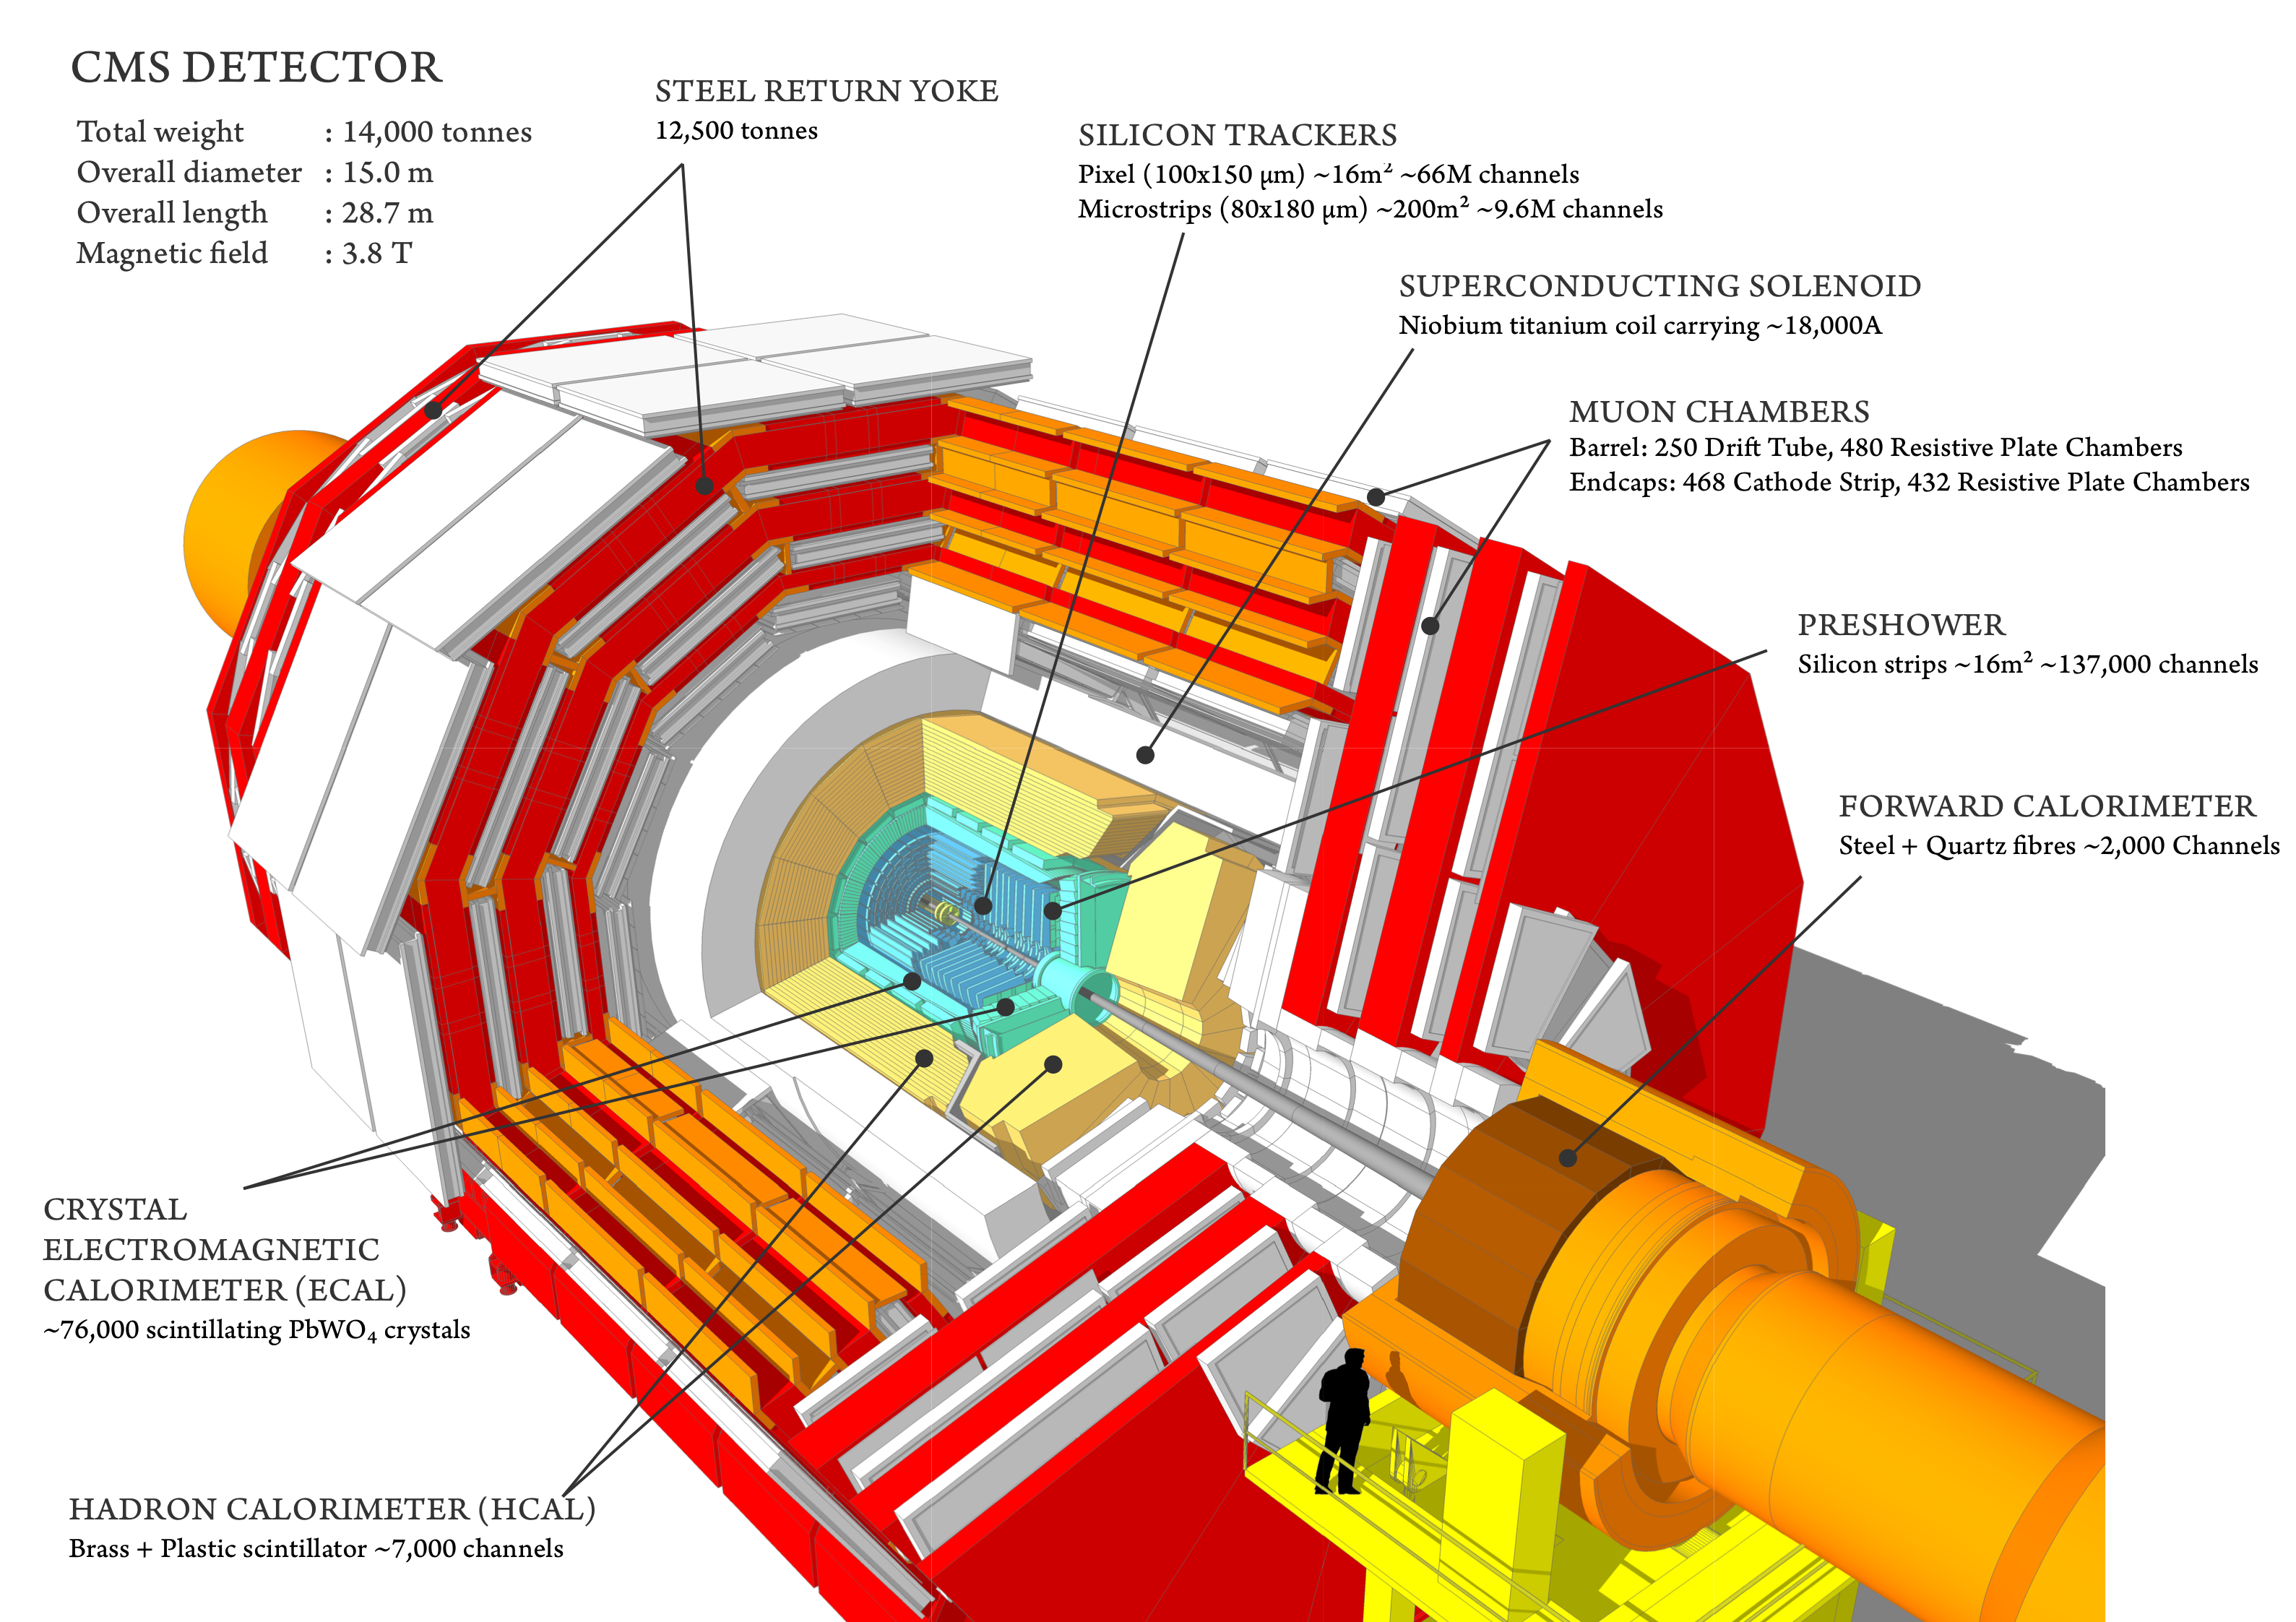
\includegraphics[width=\textwidth]{images/cms_structure.png}
    \caption{Sectional view of the CMS detector. The LHC beams travel in opposite directions along the central axis of the CMS cylinder colliding in the middle of the CMS detector. Image retrieved from http://cms.web.cern.ch/news/cms-detector-design}
    \label{fig:cms_structure}
\end{figure}
\begin{enumerate}
    \item \textbf{Tracker} to trace the footprint of charge particle by beginning at the hitting of the closest layer which is pixel detector and following by multiple layer of strip detector to gain more precision of particle track that are correspond to momentum of the particle
    \item \textbf{Electromagnetic Calorimeter (ECAL)} measure the momentum of leptons (especially electron) and photon where the main interaction obviously is electromagnetic interaction
    \item \textbf{Hadron Calorimeter (HCAL)} has been designed for measure the energy of haronic particle where it also has QCD interaction rather than only electromagnatic
    \item \textbf{Superconducting Solenoid} for generate a nearly-uniform magnetic field inside of the cylindrical shape and definitely charge particle turn their heading around where it propagate in the outside of this radius like a muon track in Figure \ref{fig:cms_slide}
    \item \textbf{Muon Detectors} is one of the most important sub-detector for measuring the muon momentum and the track of them by also take the footprint tracking system into account to get more precise information which is also the most important task of CMS detector
\end{enumerate}
\begin{figure}[h!]
    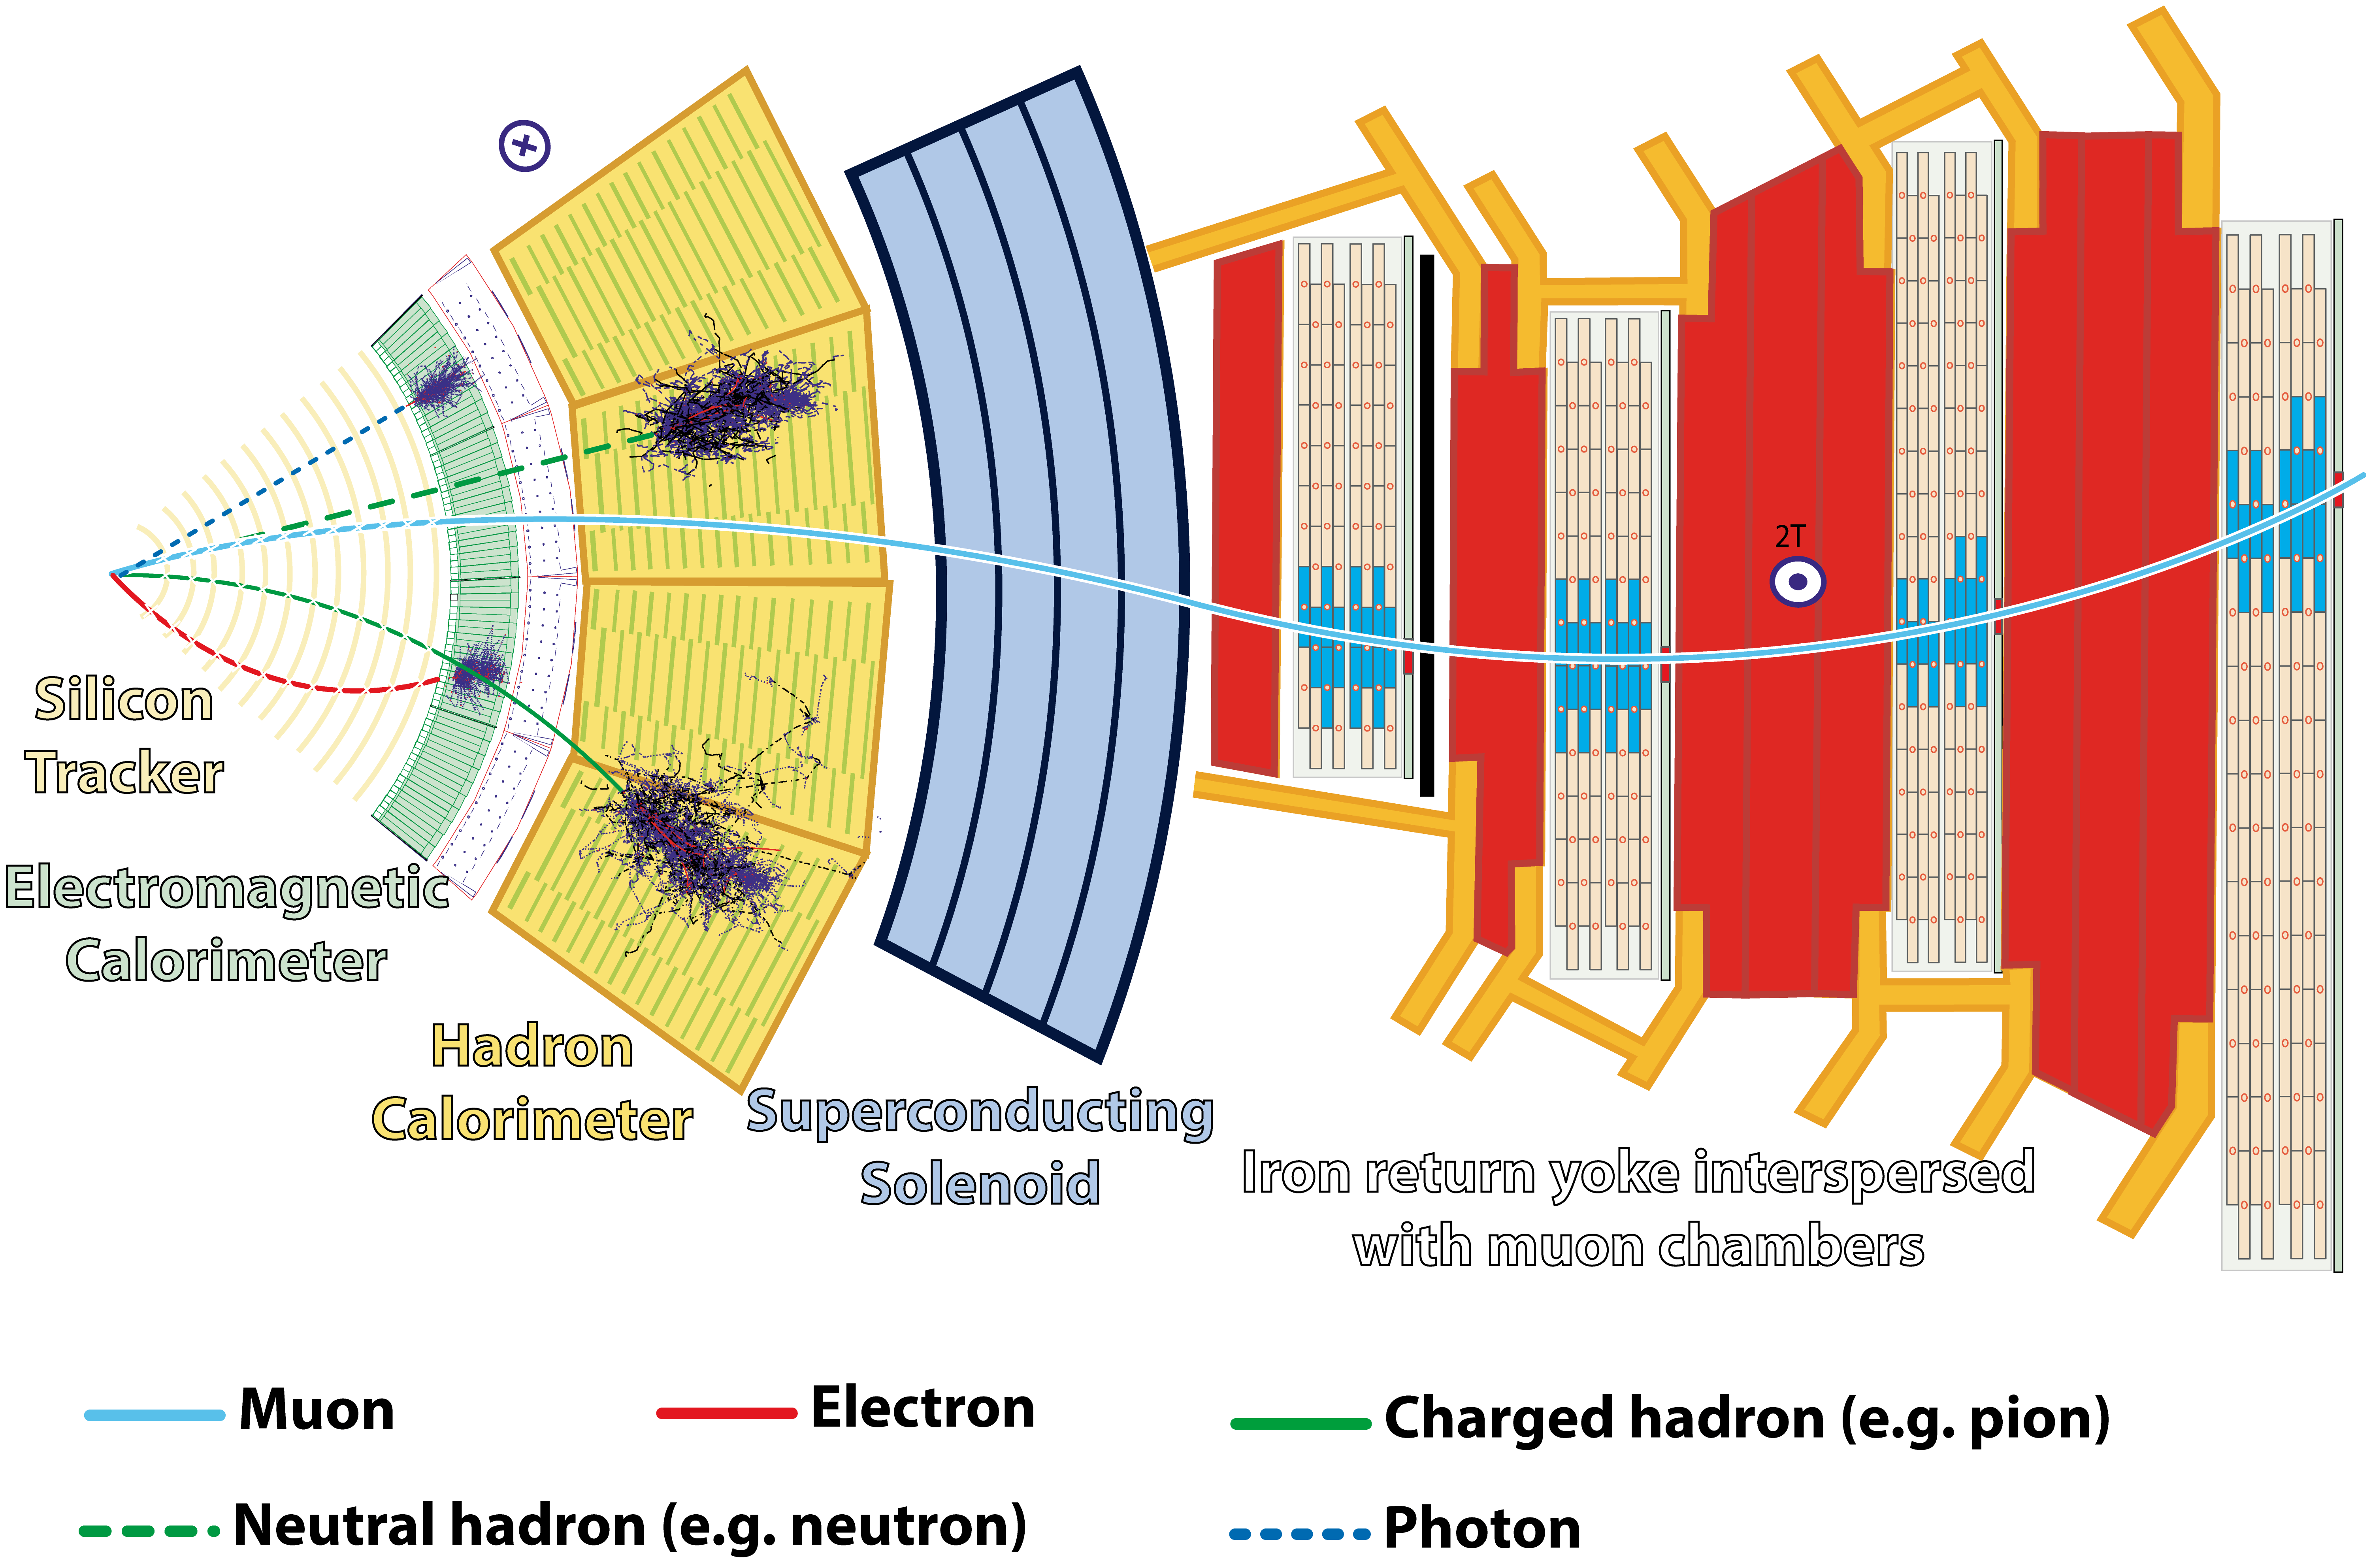
\includegraphics[width=\textwidth]{images/cms_slide.png}
    \caption{Onion-like crossection of CMS. Image retrieved from \cite{cms_onion}}
    \label{fig:cms_slide}
\end{figure}


%%%%%%%%%%%%%%%%%%%%%%
%     CMS-DAQ
%%%%%%%%%%%%%%%%%%%%%%

% \section{Data Acquisition (DAQ)}


% Figure \ref{fig:cms_structure} \cite{cms_daq} According to seminal research by \cite{Reference1}, lorem ipsum dolor sit amet.  However, this result was already known in the 1990s \citep{Reference2,Reference3}.  % Note the use of \cite{} and \citep{}


% \begin{figure}[ht]
% 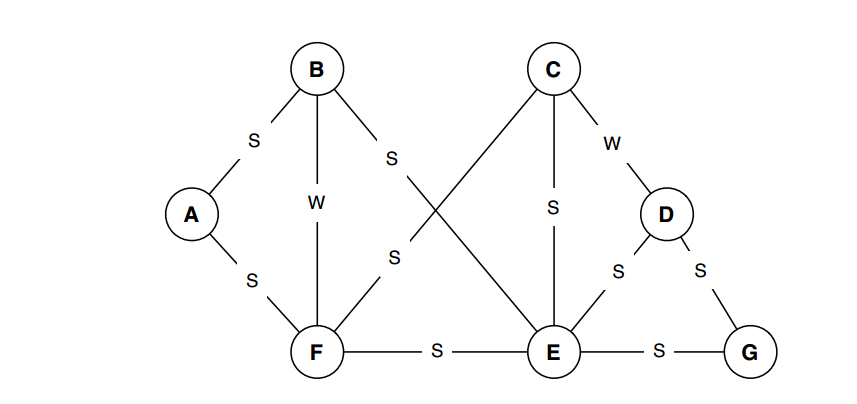
\includegraphics[width=15cm]{figures/figure1.png}
% \caption{A simple figure in \LaTeX. Reproduced from http://tinyurl.com/nqtrlj5 with the permission of the copyright owner.}
% \label{fig:graph}
% \end{figure}


% See Figure \ref{fig:graph}.


% % \section{A Section that Contains a Table}

% \begin{table}[ht]
% \center
% \begin{tabular}{cc|c}
% A & B & A XOR B\\
% \hline
% 0 & 0 & 0\\
% 0 & 1 & 1\\
% 1 & 0 & 1\\
% 1 & 1 & 0\\
% \end{tabular}
% \caption{A simple table in \LaTeX.}
% \label{tab:xor}
% \end{table}




%%%%%%%%%%%%%%%%%%%%%%
%     CMS-DQM
%%%%%%%%%%%%%%%%%%%%%%

\section{Data Quality Monitoring (DQM)}

CMS team also provide the tools for automate data acquisition as \cite{cms_daq}. 